\documentclass{article}
\usepackage[utf8]{inputenc}
\usepackage{amsfonts} 

\title{Robustness of Gaussian Process}
\author{Shiyu Zhang }
\date{}

\usepackage{natbib}
\usepackage{graphicx}

\begin{document}

\maketitle

\section{Introduction}
In this paper, our goal is to study the relationship between an input random variable $X \in \mathbb{R}^d$  and the corresponding output random variable $Y \in \mathbb{R}$ in regression problems. It is important to note that $Y$ is \emph{continuous} as we are only dealing with regressions. The learning of a relationship between $X$ and $Y$ is accomplished by estimating a mapping $f\colon \mathbb{R}^{d} \to \mathbb{R}$ between them. (We refer to function and mapping interchangeably in this paper.) \vspace{5mm}\\
As we want our estimation to be as close as possible to the true relationship between $X$ and $Y$, we may want to consider as many mappings as possible during our estimation. This is where Gaussian Process ($\mathcal{GP}$) comes in handy as a practical way for estimation and computation. $\mathcal{GP}$ incorporates a Bayesian approach into our learning where we give all possible mappings a prior probability and after observation of data, giving an updated version of them which we called the posterior distribution. One may wonder how it is computationally practical to consider all possible mappings which are definitely infinite. The marginalisation property or consistency of $\mathcal{GP}$ allows us to achieve that as $\mathcal{GP}$ helps generalize all the mappings and provides specific properties for us to study. Basically, $\mathcal{GP}$ is a collection of infinite number of random variables (the mappings), any finite number of which jointly follows a Gaussian distribution which can be completely determined by its mean and covariance function. Therefore, under $\mathcal{GP}$, following from the marginalisation property, we have $f \sim \mathcal{GP}(m(\mathbf{x}), k(\mathbf{x}, \mathbf{x'}))$ where $m(\mathbf{x})$ is the mean function and $k(\mathbf{x}, \mathbf{x'})$ = cov($f(\mathbf{x}),f(\mathbf{x'})$) is the kernel or covariance function equivalently. We use the name kernel because we can perform the kernel trick which allows us to practically compute the covariance function. \vspace{5mm}\\
As we can see, when we are estimating the mapping $f$ between $X$ and $Y$, we rely on the kernel, which completely specifies the distribution of mappings together with the mean function, to successfully capture the important properties underlying the data such as mean, smoothness, length-scale and etc. Hence, it is important in choosing our kernel wisely to uncover close-to-reality properties of the mapping. Therefore, in this paper, our interest lies in examining the impact of different kernels together with the different specification of hyperparameters for each kernel on the performance of our $\mathcal{GP}$ model. We will introduce some examples of kernels together with their respective hyperparameters and illustrate the impact of different kernels and hyperparameters on the estimation of mappings through comparison of graphs with the same set of pseudo-data.
\begin{itemize}
    \item Squared Exponential (SE) or Radial Basis Function (RBF) Kernel:\vspace{5mm}
    
    \centerline{$k_{SE}(\mathbf{x},\mathbf{x'}) = \sigma^2$exp((-$\frac{1}{2l^2}(\mathbf{x}-\mathbf{x'})^2$)}\vspace{5mm}
    
    It is usually the default kernel for $\mathcal{GP}$ models with two hyperparameters:
    \begin{itemize}
        \item The length-scale $l$ determines the length of the 'wiggles' in your function. A simple way to visualize in  2-D is to think how many units the value fluctuates in the y-direction as you move one unit in the x-direction.
        \item The variance $\sigma^2$ is a scaling factor in front determining how much in average the true function lies away from the mean function $m(\mathbf{x})$. 
    \end{itemize}\vspace{5mm}
    \item Rational Quadratic (RQ) Kernel: \vspace{5mm}\\
    \centerline{$k_{RQ}(\mathbf{x},\mathbf{x'}) = \sigma^2(1+\frac{(x-x')^2}{2\alpha l^2})^{-\alpha}$}
    This kernel is equivalent to adding many SE kernels with different length-scales together. 
\end{itemize}


\begin{figure}
\centering
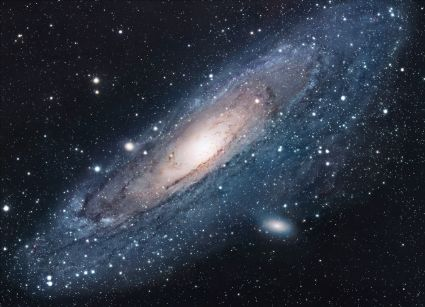
\includegraphics[scale=1.7]{universe}
\caption{The Universe}
\label{fig:universe}
\end{figure}

\section{Conclusion}
``I always thought something was fundamentally wrong with the universe'' \citep{adams1995hitchhiker}

\bibliographystyle{plain}
\bibliography{references}
\end{document}
